% Copyleft 2010, Lukas Prokop
\documentclass[11pt,a4paper]{article}

% PACKAGES
\usepackage[utf8]{inputenc}
\usepackage{ngerman}
\usepackage{bibgerm}

\usepackage{amssymb}
\usepackage{amsmath}
\usepackage{amsthm}
\usepackage{textcomp}
\usepackage{wasysym} % diameter

\usepackage[sf]{titlesec}
\usepackage{fullpage}
\usepackage{booktabs}
\usepackage{fancyhdr}

\usepackage[dvips,pdftex]{geometry}
\usepackage{graphicx}
\usepackage{pstricks}
\usepackage{pst-node}
\usepackage{pst-plot}

\usepackage[unicode,pdfborder={0 0 0}]{hyperref}
\usepackage{boxedminipage}
\usepackage{lastpage}
\usepackage{multicol}
\usepackage{units}
\usepackage{eurosym}
\usepackage{ifthen}
\usepackage{xifthen}
\usepackage{listings}
\usepackage{pifont}

% Document Configuration
\pagenumbering{arabic} % Alph, alph, arabic, Roman, roman
%\pagestyle{myheadings}
\pagestyle{plain}
\setcounter{tocdepth}{2}
\parindent0mm
\parskip2mm
%\headheight10mm
%\headsep10mm
\setlength{\unitlength}{1cm}
\renewcommand{\thefootnote}{\arabic{footnote}} % not happy with other ones :-/
\renewcommand{\theequation}{\alph{equation}}

% Aliases
% - general
\newcommand{\mathsymspace}[1]{{\hskip3pt}#1{\hskip3pt}}
\newcommand{\cmd}[1]{{\tt #1}}
\newcommand{\life}[2]{* #1 $\dagger$ #2}
\newcommand{\md}{Mitschrift der }
\newcommand{\TODO}{\fbox{\clock \color{blue} TODO}}
\newcommand{\bs}{\textbackslash}
\newcommand{\failmark}{\ding{55}}
\renewcommand{\tilde}{\textbf\texttildelow}

% financial
\newcommand{\cur}{.--\hspace{3pt}}
\newenvironment{tkonto}[1]{
    \begin{table}[!th]
      \caption{#1}
      \begin{tabular}{c | c}
        \hline
          Soll    & Haben \\
        \hline
}{
      \end{tabular}
    \end{table}
}

% - math
% --- space
\newcommand{\mathspace}{\hspace{20pt}} % n=1; \mathspace \frac{1}{n}
\newcommand{\abs}[1]{\hspace{3pt}| #1 |\hspace{3pt}}
\newcommand{\Arg}[1]{\textrm{Arg}(#1)}
\DeclareMathOperator{\arccot}{arccot}

% --- functions
%\newcommand{\mod}[1]{\bmod{#1}}
\newcommand{\eul}[1]{{\varphi}(#1)}
\newcommand{\vect}[2]{ \left ( \begin{array}{c} #1 \\ #2 \end{array} \right ) }
\newcommand{\ggt}[2]{\textrm{ggT}(#1, #2)}
\newcommand{\divides}{\hskip1pt\mid\hskip5pt}
\newcommand{\ggT}[2]{\text{ggT}(#1, #2)}
%\renewcommand{\binom}[2]{\begin{pmatrix} #1 \\ #2 \end{pmatrix}}
\newcommand{\maximum}[2]{\textrm{max}(#1, #2)}
\newcommand{\minimum}[2]{\textrm{min}(#1, #2)}
\newcommand{\set}[1]{\Big\{#1\Big\}}

% --- symbols
\newcommand{\ra}{\rightarrow}
\newcommand{\Ra}{\Rightarrow}
\newcommand{\la}{\leftarrow}
\newcommand{\La}{\Leftarrow}
\newcommand{\lra}{\Leftrightarrow}
\newcommand{\average}{\diameter}
\renewcommand{\phi}{\varphi}

% --- complex numbers
\newcommand{\comp}[1]{\overline{#1}}
\newcommand{\conj}[1]{#1 *}

% --- boolean
\newcommand{\andsym}{\mathsymspace{$ \land$}}
\newcommand{\orsym} {\mathsymspace{$ \lor $}}
\newcommand{\notsym}{\mathsymspace{$ \neg $}}
\newcommand{\true}{\hspace{1pt}\text{W}\hspace{1pt}}
\newcommand{\nomathtrue}{\hspace{1pt}W\hspace{1pt}}
\newcommand{\false}{\hspace{3pt}\text{F}\hspace{3pt}}
\newcommand{\nomathfalse}{\hspace{3pt}F\hspace{3pt}}

% - pattern.tex related
% --- general
\newcommand{\linerule}{\hrule{\textwidth}}
\newtheoremstyle{area}
    {6pt}{6pt}{\normalfont}
    {0pt}{\bfseries}{.\hspace{10pt}}{ }{#1}
\theoremstyle{area}
%\theoremstyle{plain}

% --- VO stuff
\newtheorem{mathdef}{Definition}
\newcommand{\question}[1]{\textbf{Q: }#1 \par}
\newcommand{\answer}[1]{\textbf{A: }#1 \par}
\newcommand{\quoded}{
    \parbox{\textwidth}{
        \centering{
            \textsc{
                \small{
                    --- quod erat demonstrandum. ---
                }
            }
        }
    }
}

% --- events
\newtheorem{homework}{Hausübung}
\newtheorem{exercise}{Übung}
\newtheorem{project}{Projekt}

% --- scriptum-note interaction
\newtheorem{note}{Notiz}
\newtheorem{topic}{Thema} % Topic, they are talking about
\newtheorem{chapter}{Kapitel} % Chapter in scriptum
\newcommand{\noteref}{\textbf{Siehe in Notizblättern.}\par}
\newcommand{\scriptref}[1][]{\textbf{Vergleiche im Skriptum.} #1} % TODO
\newcommand{\abbr}[2][]{
  \ifthenelse{\isempty{#1}}{
    \textbf{Abkürzung #1.} \par
  }{
    \textbf{Abkürzung #1 = #2} \par
  }
}
\newcommand{\term}[2][]{
  \ifthenelse{\isempty{#1}}{
    {\textbf{Begriff.}~''#2''}\par
  }{
    \textbf{Begriff~''#1''}~=~#2\par
  }
}

% --- design, layout
\renewcommand{\epsilon}{\varepsilon}


\author{Lukas Prokop}
\title{Sammlung der Probleme aus der LV GDI \\
    \small{Grundlagen der Informatik} \\
    \small{Lehrveranstaltung von Prof. Slany Wolfgang}
}
\date{10.12.21 -- 10.01.07}

\begin{document}
\maketitle

\section{Turingmaschine}

\emph{Angabe:} Es sei ein Eingabeband mit einer unbekannten Anzahl (größer
0) von Einsern links von genau einer Null gegeben. Der Rest des Bandes ist
mit 2 gefüllt. Der Cursor steht auf der ersten Eins.

\emph{Frage:} Programmiere eine Turingmaschine, die alle Einsen mit
Zweien überschreibt. Weiters soll die Anzahl der Einsen verdoppelt an
die rechte Seite der Null geschrieben werden. Die alten Einsen müssen
mit Zweiern überschrieben werden. Am Programmende soll sich der Cursor
auf der Null befinden.

\emph{Beispiel I/O:}
\begin{verbatim}
  Input:  ... 22211110222222222 ...
  Output: ... 22222220111111112 ...
\end{verbatim}

\section{Komplexitätstheorie -- Landau-Notation}

\emph{Angabe:} Gesucht ist eine Ordnung folgender Funktionen in n.
    Gib dabei jeweils eine möglichst langsam wachsende Funktion an:

\newcommand{\OL}{\mathcal{O}}
\newcommand{\landau}{\OL ( \hspace{60pt} )}
\[
    43^{503} = \landau
\] \[
    27 \log{n} = \landau
\] \[
    10 \log{2n} - 7 = \landau
\] \[
    13n + 8\log{3n} = \landau
\] \[
    24n \log{n} - 7n = \landau
\] \[
    17n^2 + 100n\log{1000n} = \landau
\] \[
    27n^{60} + 1^{2n} = \landau
\] \[
    (n^2 + 3n - 27)^7 = \landau
\] \[
    n^\pi  + \pi^{n-1} = \landau
\] \[
    (-2n)^{10} + \Big(\frac{1}{2}\Big)^n = \landau
%\] \[
%    42n^8 + 102^9 + 14n^k = \landau
%\] \[
%    (e^{i\pi})^{2n} = \landau
%\] \[
%    57n^{88} + 1.03^{1.03n} = \landau
%\] \[
%    (e^3 \cdot 38)^{7e} = \landau
\]

\emph{Lösungen (der Reihenfolge nach):}
\[
    \OL(1), \OL(\log{n}), \OL(\log{n}), \OL(n), \OL(n\log{n}),
    \OL(n^2), \OL(n^{60}), \OL(n^{14}), \OL(\pi^{n-1}), \OL(n^{10})
\] %\[
%    \OL(n^8 \text{ für } k <= 8; n^k \text{ für } k > 8), \OL(1),
%    \OL(1.03^{1.03n}), \OL(1)
%\]

\section{Collatz' Problem}

Dieses Beispiel ist in dieser Form nicht in der VO vorgekommen; es soll
nur als Übung dienen. Ursprünglich stammt es aus
projecteuler\footnote{\url{http://projecteuler.net/index.php?section=problems&id=14}}.

\emph{Angabe:} Die folgende iterative Zahlenfolge ist für die Menge der
    positiven Ganzzahlen definiert:

\begin{equation}
  (n \text{ ist gerade:}) n \mapsto n / 2
\end{equation}
\begin{equation}
  (n \text{ ist ungerade:}) n \mapsto 3n + 1
\end{equation}

Nutzen wir diese Folgendefinition mit der Zahl 13 als Startwert, entsteht
die Kette:

\[
    13 \ra 40 \ra 20 \ra 10 \ra 5 \ra 16 \ra 8 \ra 4 \ra 2 \ra 1
\]

Diese Kette enthält 10 Elemente. Es wurde noch nicht bewiesen, aber es ist
anzunehmen, dass jede beliebige positive Ganzzahl als Startwert nach Ablauf
des Algorithmus zu einer 1 führt.

\emph{Frage:} Schreibe ein Programm in deiner Lieblingssprache, welches mit
    einer Laufzeit von maximal 10 Sekunden die Frage beantwortet: Welcher
    Startwert unter 1 Million, erzeugt die längste Kette?

\emph{Lösung:} Die Zahl 837799 produziert eine Zahlenkette von 525 Zahlen.

\section{Logik -- The Island of Knights and Knaves}

Erklärungen in den Aufzeichnungen der VO vom 09.11.2010

\begin{itemize}
  \item Knights always say the truth.
  \item Knaves always lie.
  \item You meet two people (A and B) on the Island, each of whom is
    either a knight or a knave.
  \item A says ''I am a knave or B is a knight''
\end{itemize}

\emph{Lösung:} Remember, that the first OR (''either a
    knight or a knave.'') is a XOR and direct speech refers to a
    logical OR (''I am a knave or B is a knight''). Both are knights.

\section{Logik -- The Island II}

Erklärungen in den Aufzeichnungen der VO vom 09.11.2010

\begin{itemize}
  \item Once again, there are two persons named A and B, both of whom are
    either a knight or a knave.
  \item A says ''Either I am a knave or else two plus two equals five''
  \item What would you conclude?
\end{itemize}

\emph{Lösung:} ''Either or'' equals to XOR in logic. So the answer is
    this situation is not possible.

\section{Logik -- Three's a crowd}

Erklärungen in den Aufzeichnungen der VO vom 09.11.2010

\begin{itemize}
  \item Again we have three people, A, B, C, each of whom is either a
    knight or a knave. A and B make the following statements:
  \item A: ''All of us are knaves''
  \item B: ''Exactly one of us is a knight''
  \item What are A, B, C?
\end{itemize}

\emph{Lösung:} A is a knave. B is a knight. C is a knave.

\section{Logik -- Three's a crowd-pleaser}

Erklärungen in den Aufzeichnungen der VO vom 11.11.2010

\begin{itemize}
  \item Suppose instead, A and B say the following:
  \item A: ''All of us are knaves''
  \item B: ''Exactly one of us is a \textbf{knave}''
  \item Can it be determined what B is?
    Can it be determined what C is?
\end{itemize}

\emph{Lösung:} Nope. Neither A nor B.

\section{Logik -- Short and Sweet}

\begin{itemize}
  \item Suppose A says, ''I am a knave, but B isn't''
  \item What are A and B?
\end{itemize}

\emph{Lösung:} A and B are knaves.

\section{Logik -- Another Trio}

\begin{itemize}
  \item We have three inhabitants A, B and C, each of whom is a knight
    or a knave. A and B make the following statements:
  \item A: B is a knave.
  \item B: A and C are of the same type.
  \item What is C?
\end{itemize}

\emph{Lösung:} There are two configurations of A, B and C. In those cases,
    C is a knave.


\section{Logik -- The Final Trio}

\begin{itemize}
  \item Again three people A, B and C.
  \item A says ''B and C are of the same type''.
  \item Someone then asks C, ''Are A and B of the same type?''
  \item What does C answer?
\end{itemize}

\emph{Lösung:} Yes. There are 4 possible configurations.

\section{Logik -- The power of logic}

\begin{quote}
  This time you come across just one inhabitant lazily lying in the sun.
  You remember that his first name is either Edwin or Edward, but you
  cannot remember which. So you ask him his first name and he answers
  ''Edward''.
\end{quote}

\emph{Frage:} What is his first name?
\emph{Lösung:} Well actually\dots he is lying\dots in the sun.

\section{Logik -- Boolsche Terme lösen}

Dieses Beispiel kam nicht in der Vorlesung vor und ist eine Eigenkreation.

\emph{Aufgabe:} Löse die folgenden Terme für die Konfiguration
    $(A=True, B=True, C=False, D=True)$.

\[
    (((A \land B) \ra C) \lor (\neg C) \land (A \lor A \land B))
\] \[
    (A \land B \lor (\neg C) \land (D \ra A) \land (\neg B))
\]

\section{Logik -- Eigene boolsche Terme}

Dieses Beispiel kam nicht in der Vorlesung vor und ist eine Eigenkreation.

\emph{Aufgabe:} Vereinfache die Terme so weit wie möglich:

\[
    (((A \lor B) \lor B) \land (C \lor True))
\] \[
    (A \land B \land C \lor A \lor True)
\] \[
    ((\neg A \lor B) \lor (A \ra B))
\] \[
    (\neg \neg True \land True) \lor (False \lor True) \land
        (A \lor False) \lor (B \land True) \land C \lor D
\]

Baue nur mithilfe von NAND-Gattern eine Schaltung, die ein XOR simuliert
(zwei Eingänge mit True oder False und ein Ausgang mit einem Verhalten wie
XOR).

\section{Logik -- Portia Part One}

Die Lösung dieser Aufgabe wurde in der VO vom 18.11.2010 behandelt.

\emph{Note:} The problem's solution was given in SQL.

\begin{quote}
  There questions were taken from Raymon Smullyan's book What is the Name
  of this Book?, Prentice Hall, 1978.

  In Shakespeare's Merchant of Venice Portia had three caskets (gold, silver
  and lead) inside one of which was Portia's portrait. The suitor was to
  choose one of the caskets, and if he was lucky enough (or wise enough),
  to choose the one with the portrait, then he could claim Portia as his
  bride. On the lid of each casket was an inscription to help the suitor
  choose wisely.

  Now suppose Portia wished to choose her husband not on the basis of
  virtue, but simply on the basis of intelligence. Thus, she asks her
  suitors a riddle.

  Here is Portia's first riddle. She has the caskets inscribed as follows.
  Portia explains that at least one the statements is true and at least
  one is false.
\end{quote}

\begin{description}
  \item[gold] The portrait is not in the silver casket.
  \item[silver] The portrait is not in this casket.
  \item[lead] The portrait is in this casket.
\end{description}

\emph{Lösung:} The portrait is in the golden casket.

\section{Logik -- Portia II}

Die Lösung dieser Aufgabe wurde in der VO vom 18.11.2010 behandelt.

\emph{Note:} The problem's solution was given in SQL.

\begin{quote}
  Portia II (daughter of Portia) has the same problems as her mother
  selecting a suitable suitor. She has the following descriptions
  put on her caskets.

  Portia explained that no lid contains more than one false statement.
\end{quote}

\begin{description}
  \item[gold]
    \begin{itemize}
      \item The portrait is not in here.
      \item The artist of the portrait was born in Venice.
    \end{itemize}

  \item[silver]
    \begin{itemize}
      \item The portrait is not in the gold casket.
      \item The artist of the portrait was born in Florence.
    \end{itemize}

  \item[lead]
    \begin{itemize}
      \item The portrait is not in here.
      \item The portrait is in the silver casket.
    \end{itemize}
\end{description}

\emph{Lösung:} The portrait is in the silver casket.

\section{Logik -- Portia III}

Die Lösung dieser Aufgabe wurde in der VO vom 23.11.2010 behandelt.

\emph{Note:} The problem's solution was given in SQL.

\begin{quote}
  Portia III has her caskets made by craftsmen from Florence called
  Bellini and Cellini. Bellini always puts a true statement on the boxes
  he makes and Cellini always inscribes a false statement.

  To make things more exciting, Portia III uses a dagger instead of a
  portrait. The chances for the suitor are 2 out of 3 now, but if he
  chooses the dagger, the consequences are serious. The suitor has to
  be sure he chooses one of the two caskets without the dagger.

  The caskets are inscribed:
\end{quote}

\begin{description}
  \item[gold] The dagger is in this casket.
  \item[silver] This casket is empty.
  \item[lead] At most one of these three caskets was fashioned by Bellini.
\end{description}

\emph{Lösung:} There are two solutions. The dagger is missing in the
    gold or the silver caskets.

\section{Logik -- Einstein Problem}

Dieses Beispiel war Teil der Angabe 3. Die Lösung dieses Beispiels war
in SQL zu formulieren.

\begin{quote}
  Es gibt 5 Häuser mit je einer Farbe. In jedem Haus wohnt eine Person
  mit einer Nationalität. Jeder Hausbewohner bevorzugt eine
  bestimmtes Getränk, raucht eine bestimmte Zigarettenmarke und hat ein
  bestimmtes Haustier. Keine der 5 Personen trinkt das gleiche Getränk,
  raucht die selbe Zigarettenmarke oder hält das gleiche Tier wie
  einer seiner Nachbarn
\end{quote}

Es gelten die folgenden Bedingungen:

\begin{itemize}
  \item Der Brite lebt im roten Haus.
  \item Der Schwede hält einen Hund.
  \item Der Däne trinkt gerne Tee.
  \item Das grüne Haus steht links vom weißen Haus.
  \item Der Besitzer des grünen Hauses trinkt Kaffee.
  \item Die Person, die Pall Mall raucht, hält einen Vogel.
  \item Der Mann, der im mittleren Haus wohnt trinkt Milch.
  \item Der Besitzer des gelben Hauses raucht Dunhill.
  \item Der Norweger wohnt im ersten Haus.
  \item Der Malboro Raucher wohnt neben dem, der eine Katze hat.
  \item Der Mann, der ein Pferd hat, wohnt neben dem, der Dunhill raucht.
  \item Der Winfield Raucher trinkt gerne Bier.
  \item Der Norweger wohnt neben dem blauen Haus.
  \item Der Deutsch raucht Rothmanns.
  \item Der Malboro Raucher hat einen Nachbarn, der Wasser trinkt.
\end{itemize}

\emph{Frage:} Wer hat den Fisch als Haustier?

\emph{Lösung:} Der Deutsche.

\section{RegEx -- Analyse}

Die Lösung dieser Aufgabe wurde in der VO vom 25.11.2010 behandelt.

\emph{Angabe:} Gegeben sei der folgende Reguläre Ausdruck:

\begin{center}
  \texttt{((ab?)+(aa|b)*)+}
\end{center}

\emph{Frage:} Werden die folgenden Zeichenkette gematcht?

\begin{itemize}
  \item \texttt{ababaabb}
  \item \texttt{aabbaaba}
  \item \texttt{baaaabaaa}
  \item \texttt{aababb}
\end{itemize}

\emph{Lösung:} Ja, Ja, Nein, Nein.

\section{Regex -- Konstruktion}

\emph{Angabe:} Entwirf einen möglichst kurzen regulären Ausdruck, der genau
    jene Worte matcht, in denen die folgenden drei Bedingungen erfüllt sind:

\begin{itemize}
  \item Das Wort endet mit einem 'a'.
  \item Das erste Zeichen ist ungleich dem vorletzten Zeichen.
  \item Die Länge des Wortes ist gerade.
\end{itemize}

Ein paar valide Beispiele:

\begin{itemize}
  \item \texttt{ababba}
  \item \texttt{aaaaaaba}
  \item \texttt{babaaa}
  \item \texttt{bbaabbaa}
\end{itemize}

Ein paar invalide Beispiele:

\begin{itemize}
  \item \texttt{abbb}
  \item \texttt{baabba}
  \item \texttt{aabba}
  \item \texttt{bbaaabb}
\end{itemize}

\section{RegEx -- Analyse NFA}

Konstruiere einen Reguläre Ausdruck, der das Verhalten des folgendes
Diagramms (Abb. \ref{fig:nfa_1}) besitzt:

\begin{figure}[!ht]
  \begin{center}
    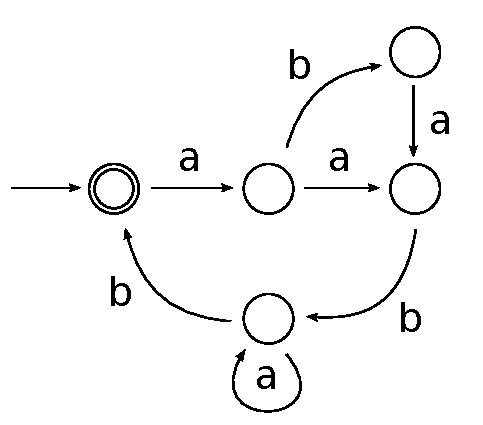
\includegraphics{nfa_1.pdf}
    \caption{Beispiel eines NFA}
    \label{fig:nfa_1}
  \end{center}
\end{figure}

\emph{Lösung:} \texttt{(ab?aba*b)*}

\section{RegEx -- Konstruktion NFA}

\emph{Angabe:} Zeichne einen deterministischen Automaten, der genau die
    Wörter akzeptiert, mit denen folgender regulärer Ausdruck matcht:

\texttt{(ab?ba*bab+|b(aba)+b+)}

Vergiss nicht mindestens einen Knoten durch einen doppelten Rand als
Terminalknoten zu kennzeichnen.

\emph{Lösung:} Abb. \ref{fig:nfa_2} (alternativ Abb. \ref{fig:nfa_3})

\begin{figure}[!ht]
  \begin{center}
    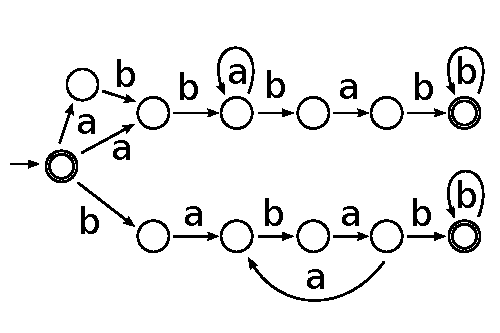
\includegraphics{nfa_2.pdf}
    \caption{NFA der Lösung}
    \label{fig:nfa_2}
  \end{center}
\end{figure}

\begin{figure}[!ht]
  \begin{center}
    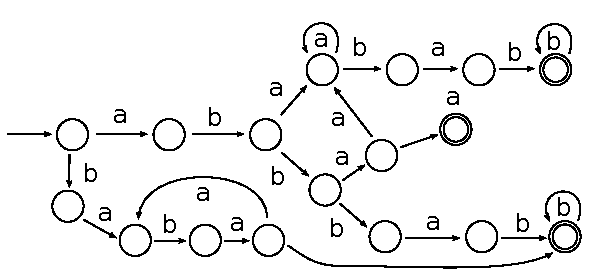
\includegraphics{nfa_3.pdf}
    \caption{2. Variante eines NFA der Lösung}
    \label{fig:nfa_3}
  \end{center}
\end{figure}

\section{Formale Grammatiken -- RegEx zu reguläre Grammatik}

Definiere eine reguläre Grammatik für folgenden regulären Ausdruck:

\begin{center}
    \texttt{ ab?ba*bab+ }
\end{center}

\emph{Lösung:}

\begin{quote}
    \texttt{S $\rightarrow$ aB \\
      B $\rightarrow$ bC \textbar\, bD \\
      C $\rightarrow$ bD \\
      D $\rightarrow$ aD \textbar\, bE \\
      E $\rightarrow$ aF \\
      F $\rightarrow$ bG \\
      G $\rightarrow$ bG \textbar\, $\varepsilon$
    }
\end{quote}

\section{Formale Grammatiken -- $a^nb^n$}

Diesen Beispiel stammt von
Wikipedia\footnote{\url{http://de.wikipedia.org/wiki/Formale\_Grammatik\#Beispiele}}
und kam in dieser Form nicht in der Vorlesung vor.

\emph{Angabe:} Konstruiere eine (kontextsensitive) Grammatik $G_1$, welche
    alle Wörter der Form $a^nb^n$ mit $n\in N_0$ beschrieben werden können.

\emph{Lösung:}
\begin{quote}
    \texttt{S $\rightarrow$ ABS \\
      S $\rightarrow \varepsilon$ \\
      BA $\rightarrow$ AB \\
      BS $\rightarrow$ b \\
      Bb $\rightarrow$ bb \\
      Ab $\rightarrow$ ab \\
      Aa $\rightarrow$ aa
    }
\end{quote}

\end{document}
